\chapter{پیش‌زمینه}
\label{chap:two}


\section{یادگیری با یک نمونه}
در یادگیری به صورت سنتی، باید داده‌ها با دو دسته آموزش و آزمون تقسیم‌بندی شوند و برای هر کلاس جدید برای دسته‌بندی باید به تعداد کافی داده وجود داشته باشد تا مدل بتواند دسته‌بندی مناسبی انجام دهد. مانند مدل کانولوشن ساده‌ای که با آن می‌توان سگ و گربه را از هم تفکیک داد. این مدل برای هر داده سگ و گربه باید تعداد قابل توجهی داده دیده باشد تا بتواند دسته‌بندی را به درستی انجام دهد. حال برای دسته‌بندی یک حیوان دیگر توسط این مدل باید داده‌های جدیدی به مدل بدهیم تا مدل بتواند آن نوع حیوان را نیز دسته‌‌بندی کند.

با بهبود ساختار شبکه یادگیرنده می‌توان نیاز فرآیند یادگیری به داده‌های زیاد را کاهش داد تا مدل بتواند با داده‌های کم نیز دسته‌بندی را انجام دهد. ارائه راهکار‌ها و روش‌هایی در کنار استفاده از شبکه‌های عصبی این امکان را به وجود آورد تا مدل فقط با دیدن یک نمونه از یک کلاس داده در فرآیند آموزش بتواند داده جدید را دسته‌بندی کند. این روش با نام یادگیری با یک نمونه شناخته می‌شود.

در این روش در فرآیند آموزش مدل به حداقل یک داده از یک کلاس داده نیاز دارد. برای جلوگیری از
\trans{بیش‌برازش}{over fitting}
در فرآیند آموزش از روش‌هایی مانند ایجاد اعوجاج در داده‌ها برای تولید داده جدید در حالات مختلف استفاده می‌شود تا مدل بتواند دسته‌بندی بهتری انجام دهد. فرآیند یادگیری با یک نمونه در مواردی پر کاربردتر است که ما تمامی کلاس‌های داده را از قبل داشته‌باشیم؛ برای مثال: در مبحث پردازش زبان طبیعی انسان، ساختار هر زبان مشخص است و زبان‌ها از یکدیگر با ساختار‌های مشخص قابل تفکیک هستند و هر زبان تعداد ثابتی قواعد و واژگان دارد. این قابلیت به ما کمک می‌کند تا بتوانیم از مدل یادگیری با یک نمونه برای کاربرد پردازش زبان طبیعی استفاده کنیم.

\begin{figure}[h]
    \centering
    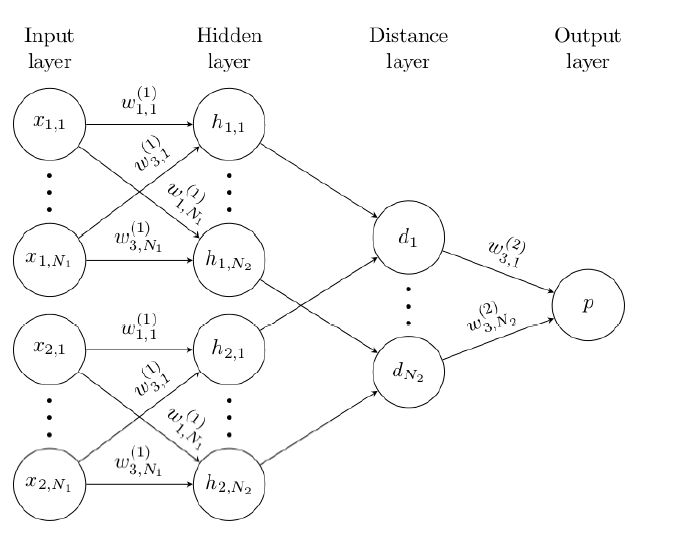
\includegraphics[width=0.5\textwidth]{img/report/simple_binary_classification_siamese}
    \caption{شبکه ساده سیامی برای دسته بند دودویی\cite{Koch}}
    \label{fig:simple-binarry-siamese}
    \centering
\end{figure}

\trans{شبکه سیامی}{Siamese network}
برای تشخیص زبان سیامی یکی از زبان‌های آسیایی است و ساختار مشخص و واژگان ثابتی را دارد ایجاد شد.این شبکه به صورت یک شبکه عصبی دو قلو است. برای دسته‌بندی این شبکه دوتایی‌های مشابه و مخالف را ایجاد می‌کند. یعنی با استفاده از شباهت‌ها و تفاوت‌های موجود درون کاراکترهای زبان آن‌ها را دسته‌بندی می‌کند در انتها هنگام دریافت نمونه جدید شبکه شباهت و تفاوت‌های این نمونه با نمونه‌های موجود را تشخیص می‌دهد و آن را در یک دسته قرار می‌دهد.

برای محاسبه تفاوت و شباهت یک معیار فاصله وزن دار L1 بین بردار‌های ویژگی استخراج شده از دو شبکه دو قلو استفاده کرده و بر اساس آن نرخ یادگیری شبکه و نحوه دسته‌بندی واژگان را مشخص کرده‌است. در شکل
\ref{fig:simple-binarry-siamese}
یک نمونه ساده از این شبکه برای دسته بندی دودویی را مشاهده می‌کنید.

شبکه سیامی یکی از شبکه‌های پر کاربرد در یادگیری عمیق است که در سیستم‌های تشخیص چهره نیز کاربرد دارد. در ادامه بررسی حملات یک مدل حمله به این شبکه نیز بررسی خواهد شد. به دلیل اینکه پایه کار و روش پیشنهادی یادگیری بدون نمونه است، در این بخش به طور مفصل آن را همراه با چند مثال بررسی می‌کنیم.


\section{یادگیری بدون نمونه}

%\cite{Wang2019}
در یادگیری بدون نمونه ما با دو نوع داده سروکار داریم. داده‌های دیده‌شده که برای آموزش مدل از آن‌ها استفاده می‌کنیم و داده‌های دیده‌نشده که مدل آموزش دیده شده باید بتواند آن‌ها را دسته‌بندی کند. داده‌های دیده‌شده، داده‌هایی برچسب خورده هستند و یک سری ویژگی‌های مشخص دارند. مدل آموزش دیده بر اساس این داده‌ها باید بتواند داده‌های دیده‌نشده را بر اساس ویژگی‌های استخراج کرده و ویژگی‌های داده‌های قبل، داده‌های جدید را دسته‌بندی کند.

فرآیند یادگیری و بررسی مدل، دو فرآیند جدا از هم هستند و داده‌های دیده‌شده و دیده‌نشده با یکدیگر اشتراکی ندارند. (به این مدل، مدل
\trans{مجموعه باز}{open-set}
گفته می‌شود.) بر این اساس می‌توان از روش یادگیری انتقالی برای یادگیری مدل‌های بر پایه یادگیری بدون نمونه استفاده کرد. در یادگیری انتقالی مدل یکبار با استفاده از داده‌های مناسب وزن‌دهی و مقداردهی شده است،‌ حال کافی‌ است مدل آماده را برای تشخیص داده‌های جدید یا در روش‌های دیگر برای فعالیت‌های دیگر به کار گرفت و نیاز نیست تا دوباره از ابتدا فرآیند یادگیری را از سر بگیریم. فرآیند یادگیری انتقالی مانند نوزاد انسان است که در ابتدا درباره محیط اطراف اطلاعات کمی دارد اما کم کم از محیط یاد می‌گیرد و از تجریبیات قبلی در یادگیری‌های بعدی نیز استفاده می‌کند.

چند حالت کلی رایج وجود دارد که استفاده از یادگیری بدون نمونه در این موارد یه ما کمک می‌کند:
\begin{itemize}
    \item
    وقتی فضای هدف به قدری بزرگ هست که همواره نمی‌توان تمامی حالات ممکن را پوشش داد؛ برای مثال: در تشخیص اشيا اطراف همواره اشیا جدید وجود دارد که در یک دسته‌بندی جدا قرار می‌گیرد.
    \item
    ممکن است نمونه‌های کلاس هدف کم‌یاب باشند و به سادگی به آن‌ها دسترسی نداشته باشیم؛ برای مثال: در تشخیص گونه‌های مختلف یک گیاه ممکن است همواره گونه‌های جدیدی پیدا شوند که تا به حال دیده نشده‌اند و یا گونه‌هایی باشند که دسترسی به آن‌ها دشوار است.
    \item
    ممکن است نمونه‌های کلاس هدف در طول زمان دچار تغییر شوند؛ مانند: نمونه‌های برند‌های مختلف پوشاک
    \item
    ممکن است داده وجود داشته‌باشد اما فرآیند برچسب گذاری هزینه‌بر باشد.
\end{itemize}

با توجه به اینکه داده‌های کلاس هدف را تا کنون ندیده‌ایم، نیاز به یک سری
\trans{اطلاعات جانبی}{auxiliary information}
داریم تا بتوانیم ارتباطی بین داده‌های آموزش و داده‌های هدف پیدا کنیم. اطلاعات جانبی باید در فضای ویژگی مرتبط با نمونه‌ها باشند تا بتوانیم به عنوان اطلاعات مناسب از آن‌ها استفاده کنیم؛ به طور مثال: در مسئله تشخیص حیوانات در صورتی که مدل ما اسب و ببر را دیده باشد می‌تواند آن‌ها را دسته‌بندی کند. حال اگر یک نمونه تصویر گورخر به مدل نشان دهیم با توجه به اینکه تاکنون مدل آن‌ را ندیده‌است باید بتوانیم با روشی به مدل بفهمانیم تا بتواند آن را نیز دسته‌بندی کند. گورخر جثه‌ای شبیه به اسب و طرحی شبیه به ببر دارد؛ این‌ها اطلاعات جانبی است که با استقاده از آن‌ها می‌توانیم بین داده‌های کلاس آموزش و هدف ارتباط برقرار کنیم. نمونه استفاده از اطلاعات جانبی در دسته‌بندی را می‌توانید در شکل
\ref{fig:attribute infromation}
مشاهده کنید.

اطلاعات جانبی مورد استفاده به طور معمول یکسری اطلاعات معنایی هستند. این اطلاعات کمکی در یک فضای جدید
(\trans{فضای معنایی}{semantic space})
شامل هر دو دسته کلاس‌های دیده‌شده و دیده‌نشده می‌شوند. فضای معنایی نیز مانند فضای ویژگی یک فضای چند بعدی است. در فضای معنایی هر کلاس با یک توصیف برداری شناخته می‌شود که به این توصبف برداری،
\trans{ضابطه کلاس}{class prototype}
گویند.

\begin{figure}[h]
    \centering
    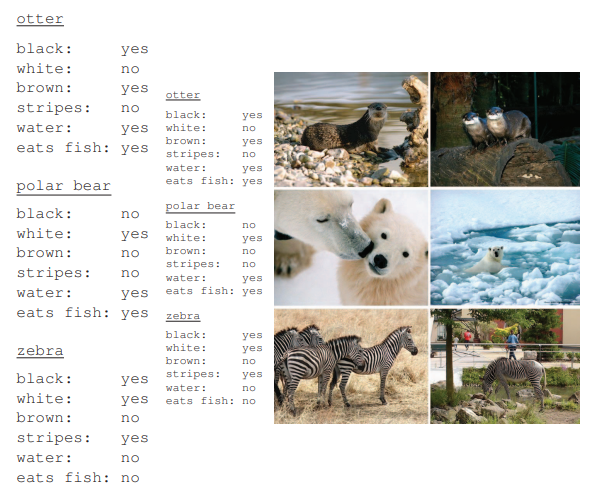
\includegraphics[width=0.8\textwidth]{img/report/sample}
    \caption{نحوه دسته بندی تصاویر توسط مدل ارائه شده\cite{Lampert2014}}
    \label{fig:attribute infromation}
    \centering
\end{figure}


به طور کلی مقالات حوزه یادگیری بدون نمونه به دو طریق بر اساس تفاوت‌های فضای معنایی و بر اساس تفاوت روش‌های استفاده شده بررسی شده‌اند.فضاهای استفاده شده در دو دسته
\trans{مهندسی شده}{Engineered} و
فضاهای
\trans{یادگرفته شده }{Learned}
و روش‌‌ها در دو دسته
\trans{بر پایه دسته‌بند}{classifier-based} و
\trans{بر پایه نمونه‌}{instance-base}
بررسی می‌شوند.\cite{Wang2019}

\subsection{فضاهای مهندسی شده}
فضا‌های مهندسی شده توسط متخصصان طراحی و متناسب با کاربرد مورد نظر استفاده شده‌اند. نمونه‌های پر کاربرد آن‌ها می‌توان به
\trans{فضای مشخصه}{Attribute}،
\trans{لغوی}{lexical} و
\trans{متنی-کلیدواژه‌ها }{text-keywords}
اشاره کرد که هر یک را متخصر توضیح می‌دهیم.

\subsubsection{فضای مشخصه}
بر اساس یک سری مشخصه‌ها ساخته شده‌اند. مشخصه‌ها ویژگی‌های سطح بالایی هستند که برای انسان یک معنا و مفهومی را تداعی می‌کنند؛ مانند: رنگ پوست، نوع زیست و محیط زندگی. این ویژگی‌ها را نمی‌توان همانند ویژگی‌های سطح پایین مانند شکل و فرم کلی بدن با استفاده از شبکه‌های عصبی کانولوشنی یاد گرفت. کاربرد این مشخصه‌ها در انتقال یادگیری است. زیرا ویژگی‌های سطح پایین برای انتقال یادگیری در یادگیری بدون نمونه ارزش چندانی ندارند. این نوع از فضا به چند دسته تقسیم بندی می‌شود: دودویی، پیوسته و نسبی.

در مقاله Lampert2014
\cite{Lampert2014}
برای دسته‌بندی حیوانات یک پایگاه داده با فضای مشخصه
\trans{پایگاه داده}{Animals with Attributes-AwA}
معرفی شده است. که شامل بیش از ۳۰۰۰۰ تصویر حیوانات در ۵۰ دسته مختلف و ۸۵ ویژگی معنایی است.

\subsubsection{فضای لغوی}
محموعه لغاتی هستند که بر پایه برچسب کلاس‌ها و داده‌هایی اند که اطلاعات معنایی دارند. مجموعه لغات استفاده شده می‌تواند WordNet باشد و برای ایجاد رابطه می‌توان روابط خواهر-برادی، والد-فرزندی و یا هر رابطه‌ قابل تعریف دیگری استفاده کرد.

\subsubsection{‌فضای متن-کلیدواژه‌ها}
این فضا بر اساس کلید‌واژه‌ها ساخته شده‌اند. کلید واژه‌ها را می‌توان از هر منبعی یا سایتی مانند ویکی‌پدیا استخراج کرد. این کلیدواژه‌ها از توصیفاتی که درباره کلاس‌های مختلف وجود دارند استخراج می‌شوند.

به طور خلاصه فضا‌های مهندسی شده توسط افراد متخصص طراحی می‌شوند و می‌توانند انعطاف‌ پذیر باشند و متناسب با فضای معنایی و قوانین دلخواه تولید شوند؛ اما نکته منفی در مورد آن‌ها این است که وابسته به یک متخصص هستیم و تلاش انسانی زیادی برای تولید آن‌‌ها باید صورت گیرد.

\subsection{فضاهای یادگرفته شده}
این فضا‌ها بر خلاف مدل قبلی توسط ماشین یاد گرفته شده‌اند. در این فضا‌ها هر بعد به تنهایی نمی‌تواند بیانگر یک معنا و مفهوم باشد و ابعاد مختلف در کنار هم معنا پیدا می‌کنند. مدل‌های ماشینی استفاده شده برای یادگیری این فضا‌ها می‌توانند مدل‌های از قبل آموزش دیده باشند یا می‌توان از پایه یک مدل را طراحی کرد. سه فضای پر کاربرد می‌توان به
\trans{جایگذاری برچسب}{Label-embedding}،
\trans{جایگذاری متن}{Text-embedding} و
\trans{نمایش تصویر}{Image-representation}
اشاره کرد.

\subsubsection{‌فضای جایگذاری برچسب}
این فضا بر اساس روش جایگذاری کلمه در پردازش زبان طبیعی ساخته شده‌است. در این روش، کلمات در فضایی از اعداد حقیقی جایگذاری می‌شوند و در نتیجه یک بردار در فضای جایگذاری به ازای هر کلمه ایجاد خواهد شد. این فضا حاوی اطلاعات معنایی است و کلماتی که حاوی معنایی نزدیک و مشابه اند در نزدیکی یکدیگر قرار می‌گیرند.
در یادگیری بدون نمونه برچسب هر کلاس یک کلمه است که می‌توان از این روش استفاده کرد.

\subsubsection{‌فضای جابگذاری متن}
این فضا شبیه به فضای متن-کلیدواژه در فضاهای مهندسی شده‌است با این تفاوت که در این فضا ماشین ارتباطات و ضوابط بین کلاس‌ها و متون را پیدا خواهد کرد.

\subsubsection{‌فضای نمایش تصویر}
در این فضا برای هر کلاس تعدادی تصویر به عنوان نمونه انتخاب خواهد شد. این نمونه‌ها به یک ماشین، داده خواهد شد تا ارتباط بین تصاویر و کلاس‌های مورد نظر را پیدا کند و از آن طریق بردارهای خروجی را یافته و ضابظه کلاس‌ها را تشکیل دهد. برای مقابله با حملات و جعل تصاویر چهره ما نیاز به تولید چنین فضاهایی هستیم.

به طور خلاصه فضاهای یادگرفته شده نیازی به یک انسان متخصص ندارند و می‌توانند ویژگی‌هایی را تولید کنند که شاید از دید متخصص پنهان بنمان که این می‌تواند یک برتری نسبت به فضای مهندسی شده باشد. از طرفی، این نکته که هر بعد این فضاها به تنهایی یک معنا و مفهوم مستقل ندارد می‌تواند یک نقطه ضعف در مقابل فضاهای مهندسی شده باشد.

\subsection{روش‌‌های بر پایه دسته‌بند}
هدف و تمرکز در این روش‌ها این است که از یک دسته‌بند برای تشخیص کلاس‌های دیده‌نشده استفاده کنیم. روش این دسته‌بند‌ها
\trans{یک در مقابل بقیه}{one versus rest}،
است که در این روش در هر تصمیم گیری برای کلاس دیده نشده یک مسئله دسته‌بندی دودویی وجود خواهد داشت. در حقیقت این روش‌ها یک سری دسته‌بند دودویی در کنار هم هستند. روش‌های ساخت دسته‌بند‌ها در ادامه آورده شده‌است. این روش‌ها در سه دسته
\trans{مبتنی بر تطابق}{Correspondence}،
\trans{میتنی بر ارتباط}{Relationship} و
\trans{مبتنی بر ترکیب}{Combination}
بررسی می‌شوند.

\subsubsection{‌روش مبتنی بر تطابق}
هدف، ساخت دسته‌بند با یافتن شباهت‌های موجود بین دسته‌بند یک در مقابل بقیه هر کلاس و ضابطه آن کلاس است. ضابطه هر کلاس یک نمایش و توصیفی از کلاس است و یافتن شباهت و تطابق بین آن و دسته‌بندی مربوط به آن کلاس به تولید دسته‌بند اصلی منجر می‌شود. برای داده‌های دیده نشده با استفاده از ضابطه کلاس و تابع تطابق یافت شده یک دسته‌بند ساخته می‌شود و کلاس جدید دسته‌بندی می‌شود.

نتطه قوت این روش ارتباطات بر پایه تابع تطابق است که به راحتی قابل یافتن است اما نقطه ضعف این روش این است که این ارتباطات را به طور صریح و واضح بیان نمی‌کند.

\subsubsection{‌میتنی بر ارتباط}
هدف، ساخت دسته‌بند بر اساس ارتباط بین کلاس‌هاست. برای یافتن ارتباط میان کلاس‌های دیده‌شده و دیده‌نشده می‌توان از ارتباط بین ضابطه کلاس‌ها و یا هر ارتباط مناسب دیگری استفاده کرد. برای کلاس‌های دیده‌نشده با استفاده از ارتباط موجود و دسته‌بند کلاس‌های دیده‌شده یک دسته بند برای هر کلاس دیده‌نشده ساخته می‌شود.

از دسته‌بندی کلاس‌های دیده‌شده می‌توان در مسائل دیگر نیز استفاده کرد و هزینه آموزش مدل را کاهش داد؛ اما، روابط بین کلاس‌ها از فضای معنایی به فضای ویژگی به طور مستقیم متنقل می‌شود که حل مسئله سازگاری از فضای معنایی به فضای ویژگی مشکل است.

\subsubsection{مبتنی بر ترکیب‌}
در این روش هر کلاس را ترکیبی از چند عنصر در نظر می‌گیریم که این عناصر در فضای معنایی وجود دارند. در حقیقت برای استفاده باید از فضاهای دودویی استفاده کرد که فضاهای معمول استفاده شده فضاهای مهندسی شده هستند. روش ساخت دسته‌بند برای کلاس‌های دیده‌نشده بدین صورت است که برای هر یک از عناصر سازنده کلاس‌ها دسته‌بند ساخته شده‌‌است سپس از آن دسته‌بند‌ها برای ساخت دسته‌بند کلاس جدید استفاده می‌کنیم.

همانند روش قبل می‌توان از دسته‌بندی‌های مورد استفاده در مسائل دیگر نیز استفاده کرد؛ اما، بهینه سازی مسئله دو مرحله‌ای آموزش دسته‌بند مشخصه و استنتاج از مشخصه به کلاس دشوار است.

\subsection{روش‌‌های بر پایه نمونه}
هدف در این روش‌‌ها ایجاد نمونه برچسب‌خورده برای کلاس‌های دیده نشده است. با استفاده از این نمونه‌ها دسته‌بند اصلی آموزش می‌بیند. با توجه به تفاوت در نحوه و منبع تولید نمونه،‌ این روش‌‌ها به سه زیر دسته
\trans{مبتنی بر تصویر کردن}{Projection}،
\trans{میتنی بر قرض نمونه}{Instance-borrowing} و
\trans{مبتنی بر سنتز}{Synthesizing}
تقسیم می‌شوند.

\subsubsection{مبتنی بر تصویر کردن‌}
تولید نمونه برای کلاس دیده‌نشده از طریق تصویرکردن نمونه‌های موجود در فضای ویژگی و ضابطه‌های موجود در فضای معنایی، به یک فضای مشترک انجام می‌شود. در فضای ویژگی با استفاده از دسته‌بند می‌توان داده‌های آزمایش را دسته‌بندی کرد. این ویژگی‌ها فقط برای داده‌های آزمایشی موجود هستند. فضای معنایی شامل ضابطه‌هایی است که هم شامل داده‌های جدید و هم شامل داده‌های آزمایش می‌شوند. می‌بایست یک ارتباط بین فضای ویژگی و فضای معنایی پیدا کنیم و با انتقال هر دو فضا و تصویر کردن در یک فضای سوم از ضابطه‌های موجود به عنوان نمونه کلاس‌های دیده نشده استفاده کنیم. با توجه به اینکه با این روش برای هر کلاس دیده‌نشده یک نمونه تولید می‌شود و فرآیند دسته‌بندی دشوار می‌شود می‌توان از روش‌های ناپارامتری مانند روش KNN استفاده کرد تا بتوان دسته‌بندی بهتری داشت.

انتخاب تابع نگاشت انعطاف پذیر است و با توجه به شرایط مسئله می‌توان دادگان مناسب انتخاب کرد؛ اما، چون برای هر کلاس دیده‌نشده یک نمونه برچسب زده وجود دارد ناچار به استفاده از روش‌های ناپارامتری می‌شویم.

\subsubsection{مبتنی بر قرض نمونه‌}
در این روش بر اساس شباهت‌های بین کلاس‌های دیده شده و دیده نشده برای کلاس‌های دیده نشده از کلاس‌های دیده‌شده نمونه قرض می‌گیریم؛ برای مثال: اگر تا کنون کلاس یوزپلنگ را ندیده‌ایم می‌توانیم از کلاس پلنگ و ببر نمونه قرض بگیریم و برای آموزش کلاس یوزپلنگ از این نمونه‌ها استفاده کنیم. این نمونه‌ها به طور کامل مانند نمونه اصلی نیستند اما به دلیل شباهت‌هایی که دارند می‌توانند برای استفاده مناسب باشند.

به دلیل گستردگی نمونه‌های قرض داده‌شده می‌توان مدل‌های دسته‌بندی نظارت شده مختلفی را استفاده کرد؛ اما، چون نمونه‌ها همان نمونه‌های کلاس‌های دیده شده هستند باعث می‌شود تا دقت پایینی در دسته‌بندی داشته باشیم.

\subsubsection{مبتنی بر سنتز‌}
در این روش برای هر کلاس دیده‌نشده یک سری نمونه برچسب‌خورده می‌سازیم و با استفاده از آن‌ها کلاس‌های دیده نشده را آموزش می‌دهیم. در حقیقت پس از ساخت نمونه برای همه کلاس‌ها مسئله به یک مسئله یادگیری ماشین نظارت شده می‌شود. برای تولید داده مصنوعی روش‌های منعددی وجود دارد؛ برای مثال: اگر فرض کنیم که کلاس‌ها از یک توزیع خاص تبعیت می‌کنند با استفاده از حدس پارامتر‌های آن توزیع برای کلاس‌های دیده‌نشده می‌توان داده‌های مصنوعی تولید کرد.

از دیگر روش‌ها می‌توان به
\trans{شبکه‌های مولد متخاصمی یا GAN}{Generative Adverserial Networks}
اشاره کرد. این شبکه‌ها از دو شبکه ساخته شده‌اند که یکی وظیفه تولید داده و دیگری وظیف صحت سنجی داده را دارد تا داده تولید شده به داده اصلی شبیه تر باشد. این شبکه‌ها در تولید داده مصنوعی از روش‌های دیگر از عملکرد و دقت بالاتری برخوردار هستند. استفاده از شبکه‌های GAN، یکی از روش‌های مرسوم برای تولید تصاویر جعلی برای دور زدن فرآیند احراز هویت سیستم‌های تشخیص چهره و گرفتن دسترسی از سیستم است.

به دلیل گستردگی نمونه‌های تولید شده می‌توان مدل‌های دسته‌بندی نظارت شده مختلفی را استفاده کرد؛ اما، چون نمونه‌های تولید شده به طور معمول از توزیع نرمال پیروی می‌کنند. می‌تواند باعث سو گیری مدل تولید شده شود.

در خارج از شرایط آزمایشگاهی کلاس‌های دیده‌شده و دیده‌نشده در ترکیب با هم هستند و به این سادگی نمی‌توان آن‌ها را جدا از هم در نظر گرفت به همین دلیل میحث
\trans{یادگیری بدون نمونه تعمیم یافته }{Generalized zero-shot learning}
مطرح می‌شود. در حل این نوع مسائل روش‌های یاد شده لزوما نتیجه مناسبی نمی‌دهند و باید به دنبال روش‌های بهتر بود.

\subsection{یک مثال}
روش‌ها و فضاهای یادگیری در یادگیری بدون نمونه در این فصل بررسی شد در ادامه یک مثال از یادگیری بدون نمونه برای دسته‌بندی حیوانات را برای فهم بهتر بررسی می‌کنیم.

مدل‌های مختلف که بر پایه روش یادگیری بدون نمونه ارائه شده‌اند می‌توانند ترکیبی از روش‌ها و فضا‌ها را داشته باشند و یا فقط متکی بر یکی از آن‌ها طراحی شده باشند. به عنوان مثال در مقاله
\cite{Lampert2014}
از فضای مشخصه استفاده کرده‌است و سعی کرده با ارائه دو روش برای یادگیری حیوانات مختلف را دسته‌بندی کند. مقاله از سه روش برای دسته‌بندی نام برده‌است و آن‌ها را با یکدیگر مقایسه می‌کند.
\trans{دسته بندی چندکلاسه مسطح}{flat multi-class classification}،
\trans{پیش بینی مشخصه به طور مستقیم}{direct attribute prediction} و
\trans{پیش بینی مشخصه به طور غیر مستقیم }{indirect attribute prediction}
به طور شهودی این سه روش در شکل
\ref{fig:learning-methods}
نشان داده شده‌اند.
به دلیل این‌که همواره نمی‌توان پایگاه داده‌ای کامل و برچسب خورده داشت نیازمند راهکار‌هایی هستیم تا تلاش انسان در جمع‌آوری و دسته‌بندی‌ داده‌ها را کم کنیم.

در شکل
\ref{fig:learning-methods}
تصویر الف، نشان دهنده روش اول است. در این روش ماشین یک بردار ثابت را یاد میگیرد. x ورودی مسئله، y برچسب‌ داده‌ها آزمایش و z برچسب داده‌هایی است که نیاز داریم آن‌ها را بیابیم. چون فرآيند یادگیری y هیچ تاثیری بر فرآیند یادگیری z ندارد پس از یادگیری‌های قبلی برای پیش بینی نمی‌توان استفاده کرد و این روش یک روش یادگیری معمولی است که قبلا نیز استفاده می‌شد و برای یادگیری z نیازمند داده‌های ورودی هستیم که با توجه به اینکه به دنبال یادگیری بدون نمونه هستیم این روش مناسب نیست.

راهکار ارائه شده برای یادگیری استفاده از ویژگی‌های معنایی سطح بالایی هستند که هرکدام برای انسان معنای خاصی دارند. این مشخصه‌ها، ویژگی‌های قابل نام‌گذاری هستند؛ مانند: رنگ، شکل، طرح بدن و عادات غذایی. استفاده از این مشخصه‌‌ها به ما کمک می‌کند تا نقش انسان را در فرآیند یادگیری کمتر کنیم و نیاز کمتری به ویژگی‌های سطح پایین تصویر داشته باشیم.

این مشخصه‌ها را می‌توان همراه با تصاویر یا همراه با دسته‌بندی‌های تصاویر درنظر گرفت و این ویژگی باعث شده است تا فرآیند
\trans{دسته‌بندی بر اساس مشخصه‌ها}{attribute-based classification}
توسط مقاله معرفی شود. در این فرآیند با توجه به اینکه دسته‌های آموزش و آزمایش جدا از هم هستند و به یکدیگر وابسته نیستند؛ می‌توان با استفاده از این صفات و
\trans{انتقال یادگیری}{transfer learning}،
بین داده‌های آموزشی، داده‌های آزمایشی را دسته‌بندی کرد. در شکل
\ref{fig:attribute infromation}
می‌توانید نحوه دسته‌بندی بر اساس صفات را مشاهده کنید.
با توجه به توضیحات ارائه شده به سراغ توضیح دو روش دیگر می‌رویم.
\begin{figure}[h]

    \centering
    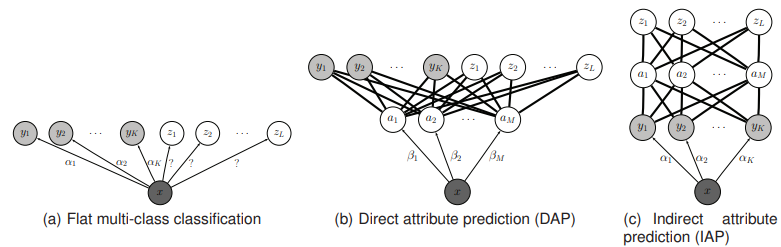
\includegraphics[width=\textwidth]{img/report/learning-methods}
    \caption{روش‌های دسته‌بندی \cite{Lampert2014}}
    \label{fig:learning-methods}
    \centering
\end{figure}
\\
در روش
\trans{پیش‌بینی مشخصه‌ به صورت مستقیم}{direct attribute prediction}
یا DAP در مرحله آموزش کلاس خروجی هر نمونه (x) برای لایه مشخصه‌ها نیز به طور قطع یک برچسب (y) مشخص می‌کند. متعاقبا می‌توان از هر روش با نظارتی استفاده کرد و پارامتر‌های هر مشخصه‌
\textsubscript{m}$\beta$
را پیدا کرد. این بدین معنی است که فرآیند یادگیری اولیه برای یادگیری مشخصه‌ها متناسب با هر نمونه و دسته‌بندی مشخصه‌ها و نمونه‌ها را می‌توان با یک روش یادگیری نظارتی ساده انجام داد. حال با استفاده از یادگیری انتقالی و استفاده از شبکه‌ای که از پیش نمونه‌ها و مشخصه‌ها آن دسته‌بندی شده‌اند برای نمونه‌های جدید که از پیش دیده نشده‌اند (داده‌های آزمون) دسته‌بندی جدیدی را فقط بر اساس لایه مشخصه‌ها وزن‌ها یا پارامتر‌هایی که شبکه تا به حال دارد و به لایه مشخصه‌ها اختصاص داده‌است، استفاده کرد و داده جدید را دسته‌بندی کرد.
\\
در روش
\trans{پیش‌بینی مشخصه‌ به صورت غیر مستقیم}{indirect attribute prediction}
یا IAP همانند روش قبل از مشخصه‌ها برای انتقال دانش بین دسته‌ها استفاده می‌کند اما اینبار مشخصه‌ها بین دولایه از برچسب‌ها قرار دارند. یک لایه برچسب‌هایی که در لایه آموزش اختصاص می‌یابند (y) و یک لایه برچسب‌هایی که باید به داده‌های جدید اختصاص پیدا کنند (z) . در مرحله آموزش پارامتر‌های لایه مشخصه‌ها توسط برچسب‌های آموزش مقدار دهی می‌شوند همانند یک مسئله دسته‌بندی چند‌کلاسه که می‌توان با یک روش نظارتی ساده نیز یادگیری را انجام داد. در مرحله آزمایش با استفاده از مقادیری که به لایه مشخصه‌ها اختصاص داده‌شده دسته‌بندی داده‌های آزمایش را صورت می‌گیرد. استفاده از لایه مشخصه‌ها به برای دسته‌بندی داده‌های آزمایش این امکان را می‌دهد تا بتوانیم عملیاتی مشابه
\trans{تنظیم}{regularization}
را انجام دهیم و فقط ترکیبات با معنی از مشخصه‌ها را ایجاد کنیم.

روش‌های یاد شده یک سری استراتژی کلی محسوب می‌شوند که می‌توانند با ترکیبی از روش‌‌های موجود مانند: یادگیری با نظارت یا رگرسیون‌ها بر روی مشخصه‌ها تصاویر یا دسته‌های تصاویر با استفاده از پارامتر‌های پیش‌بینی شده انجام شوند. در این مقاله از روش توزیع‌های احتمالاتی استفاده شده و مشخصه‌های استفاده شده را مشخصه‌هایی بله یا خیر در نظر گرفته‌است. برای مشخصه‌هایی که بله یا خیر نیستند می‌توان به جای دسته‌بندی از رگرسیون استفاده کرد.

در روش DAP برای دسته‌بندی کردن تصاویر آزمون، احتمال قطعی به دست خواهد آمد زیرا در مرحله آموزش لایه مشخصه‌ها مقادیر مناسب را اتخاذ می‌کنند و از همین مقادیر برای تصاویر آزمون نیز استفاده می‌شود. به زبان ریاضی معادلات زیر صادق است.


\begin{equation}
    p(z|x) = \sum_{a\in(0,1)^{M}} p(z|a)p(a|x)\dfrac{p(z)}{p(a^{a})}\prod_{m=1}^{M} p(a_{m}^{z}|x).
\end{equation}

\begin{equation}
    f(x) = \argmax\limits_{l=1,...,L} p(z=l|x) = \argmax\limits_{l=1,...,L} \prod_{m=1}^{M} \dfrac{p(a_{m}^{z_{l}}|x)}{p(a_{m}^{z_{l}})}.
    \label{eq:2}
\end{equation}

در روش IAP لایه مشخصه‌ها نقش یک تنظیم‌کننده را ایفا می‌کند پس به طور قطع نمی‌توان برای تشخیص لایه آزمون استفاده کرد و می‌بایست با استفاده از روابط احتمال یک احتمال میانی را حساب کرد و پس از آن از رابطه\ref{eq:2}
استفاده کرد.
\begin{equation}
    p(a_{m}|x) = \sum_{k=1}^{K} p(a_{m}|y_{k})p(y_{k}|x).
\end{equation}
\\
سه بانک اطلاعاتی استفاده شده است. در ادامه هر یک را توضیح می‌دهیم.\ref{table:Datasets}

\subsubsection{\lr{Animal with Attributes}}

این بانک اطلاعاتی به عنوان بانک اصلی استفاده شده است. این بانک شامل ۵۰ کلاس حیوانات و ۸۵ کلاس مشخصه‌های معنایی است؛ از این تعداد ۴۰ کلاس به عنوان داده‌های آموزشی و ۱۰ کلاس به عنوان داده‌های آزمایش استفاده شده است. تقسیم بندی به صورت تصادفی نیست اما سعی شده است تا توزیع داده‌ها در هر دو دسته آزمایش و آزمون به طور مناسبی صورت شود.

در کل 30475 عکس در این بانک داده وجود دارد که تعداد تصاویر برای دسته‌های مختلف حیوانات متفاوت می‌باشد. برای تسریع در محاسبات یک سری از ویژگی‌های تصاویر مانند: جنبه‌های رنگ، بافت و شکل، هیستوگرام رنگ و سایر ویژگی‌های مهم تصویر نیز به پایگاه داده اضافه شده‌و برای آموزش از روش
\lr{5 fold cross-validation}
استفاده شده‌است.

\subsubsection{\lr{aPascal-aYahoo}}

این بانک شامل دو دسته داده یکی داده‌های بانک داده PASCAL و دیگری داده‌هایی که از موتور جستجوی Yahoo استخراج شده است. ۲۰ کلاس داده در PASCAL و ۱۲ کلاس داده در Yahoo و دسته‌بندی داده‌ها در هر یک با دیگری متفاوت است پس می‌توان از داده‌های PASCAL برای آموزش و از داده‌های Yahoo برای آزمون استفاده کرد. هر تصویر ۶۴ مشخصه‌ها دودویی را شامل ‌می‌شود و همانند بانک داده قبلی برای تسریع در محاسبات یک سری از ویژگی‌های تصاویر از قبل محاسبه شده‌اند.

\subsubsection{\lr{SUN Attributes}}

این بانک زیر مجموعه‌ای از بانک داده‌
\lr{SUN Database}
که شامل 717 کلاس داده و هر تصویر شامل ۱۰۲ مشخصه‌ دودویی است. این مشخصه‌ها شامل توضیفات صحنه، شرایط نورپردازی، مواد داخل تصویر و ... است.

\begin{table}[h]
    \begin{center}
        \caption{بانک‌های اطلاعاتی\cite{Lampert2014}}
        \begin{tabular}{c|c|c|c}
            Dataset                & AwA       & aP/aY     & SUN       \\
            \hline \lr{\# Images}  & 30475     & 15339     & 14340     \\
            \lr{\# Classes}        & 50        & 32        & 717       \\
            \lr{\# Attributes}     & 85        & 64        & 102       \\
            \lr{Annotation Level}  & per class & per image & per image \\
            Annotation Type (real- & both      & binary    & binary    \\
            valued or binary) & &
        \end{tabular}

        \label{table:Datasets}
    \end{center}
\end{table}

برای ارزیابی از
\trans{ماشین بردار پشتیبان}{Support Vector Machine} یا SVM
استفاده شده‌‌است. برای روش مستقیم از یک SVM غیر خطی و برای روش غیرمستقیم از نوع
\lr{one-versus-rest}
استفاده شده‌است.
نتایج به دست آمده را در جداول\ref{table:result1} و\ref{table:result2}
مشاهده می‌کنید.


\begin{table}[h]
    \begin{center}
        \caption{تقسیم بندی پیش‌فرض داده‌ها \cite{Lampert2014}}
        \begin{tabular}{c|cc|cc|c}
            method              & DAP  & IAP  & CT-cc          & CT-H           & rnd  \\
            \hline \lr{MC acc.} & 41.4 & 42.2 & $30.7 \pm 0.2$ & $30.8 \pm 0.2$ & 10.0 \\
            classAUC            & 81.4 & 80.0 & 73.4           & 73.4           & 50.0 \\
            attrAUC             & 72.8 & 72.1 & $-$            & $-$            & 50.0
        \end{tabular}

        \label{table:result1}
    \end{center}
\end{table}
\begin{table}[h]
    \begin{center}
        \caption{تقسیم بندی داده‌ها به صورت تصادفی\cite{Lampert2014}}
        \begin{tabular}{c|cc|cc|c}
            method              & DAP            & LAP            & CT-cc          & CT-H           & md   \\
            \hline \lr{MC acc.} & $37.1 \pm 3.9$ & $34.1 \pm 5.1$ & $27.7 \pm 4.3$ & $27.3 \pm 4.0$ & 10.0 \\
            classAUC            & $80.4 \pm 3.1$ & $76.3 \pm 5.5$ & $72.4 \pm 2.7$ & $72.8 \pm 3.1$ & 50.0 \\
            attrAUC             & $70.7 \pm 3.5$ & $69.7 \pm 3.8$ & $-$            & $-$            & 50.0
        \end{tabular}

        \label{table:result2}
    \end{center}
\end{table}

%\begin{figure}[b]
%	\centering
%	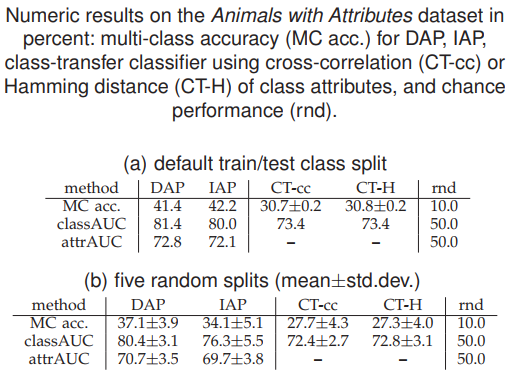
\includegraphics[width=0.5\textwidth]{img/report/results}
%	\caption{نتایج \cite{Lampert2014}}
%	\label{fig:results}
%	\centering
%\end{figure}
در روش مستقیم برای بدست آوردن مقادیر مناسب کرنل SVMاز منحنی
\trans{ROC}{Receiver Operation Characteristic}
و
\trans{میانگین سطح زیر منحنی}{AUC}
برای صفات و روش
\lr{5 fold cross-validation}
استفاده شده‌است.

منحنی یاد شده، یک نمودار برای نمایش توانایی ارزیابی یک سیستم دسته‌بندی دودویی محسوب می‌شود که آستانه تشخیص آن نیز متغیر است. که با ترسیم نسبت
\trans{نرخ مثبت صحیح}{True Positive Rate}
که به اختصار TPR نامیده می‌شود برحسب
\trans{نرخ مثبت کاذب}{False Positive Rate}
با نام اختصاری FPR، ایجاد می‌شود.

در روش غیر مستقیم مراحل مانند روش قبل است با این تفاوت که میانگین سطح زیر منحنی بر روی پیش‌بینی کلاس‌ها استفاده شده‌است.

\begin{figure}[h]
    \centering
    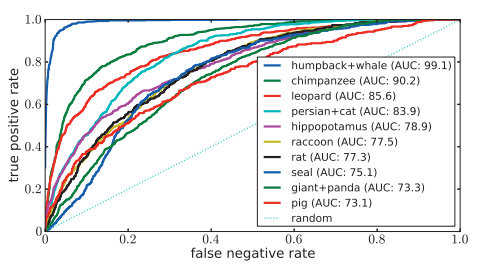
\includegraphics[width=0.6\textwidth]{img/report/ROC}
    \caption{منحنی ROC\cite{Lampert2014}}
    \label{fig:ROC}
    \centering
\end{figure}
همان‌طور که در شکل\ref{fig:ROC}
مشاهده می‌کنید. دقت روش در تشخیص برخی از دسته‌ها مانند نهنگ‌های کوهان‌دار دقت بالایی همانند روش‌های یادگیری با نظارت دارد؛ اما در مورد دسته‌بندی‌هایی مانند خوک‌هاو پاندا‌های بزرگ دقت خیلی پایینی دارد. یکی از دلایل این اتفاق شباهت‌هایی است که در این دسته‌ها رخ می‌دهد؛ به طور مثال: ظاهر پاندا‌های بزرگ، خوک‌ها و اسب‌های آبی.

به طور مشابه بر روی دو پایگاه داده دیگر نیز بررسی‌ها انجام شده‌است و نتایج را در جداول زیر مشاهده می‌کنید.

\begin{table}[h]
    \label{tab:other_result1}
    \begin{center}
        \caption{تقسیم بندی پیش‌فرض داده‌ها برای aPascal-aYahoo\cite{Lampert2014}}
        \begin{tabular}{c|ccc|cc}
            method              & DAP-I & DAP-C & IAP  & CT-H           & rnd  \\
            \hline \lr{MC acc.} & 16.8  & 19.1  & 16.9 & $16.7 \pm 0.5$ & 8.3  \\
            classAUC            & 76.9  & 76.5  & 75.4 & 64.2           & 50.0 \\
            attrAUC             & 70.6  & 73.7  & 73.1 & $-$            & 50.0
        \end{tabular}
    \end{center}
\end{table}

\begin{table}[h]
    \begin{center}
        \caption{تقسیم بندی داده‌ها برای sub attributes\cite{Lampert2014}}
        \begin{tabular}{c|ccc|cc}
            method              & DAP-I          & DAP-C          & IAP            & CT-H           & rnd  \\
            \hline \lr{MC acc.} & $18.1 \pm 1.2$ & $22.2 \pm 1.6$ & $18.0 \pm 1.5$ & $12.9 \pm 1.3$ & 1.4  \\
            \lr{level2 acc.}    & $40.2 \pm 2.1$ & $46.6 \pm 1.7$ & $41.1 \pm 2.1$ & $32.6 \pm 2.0$ & 6.2  \\
            \lr{level1 acc.}    & $74.2 \pm 4.0$ & $85.7 \pm 2.1$ & $82.1 \pm 2.5$ & $74.2 \pm 2.0$ & 33.3 \\
            \lr{class mAUC}     & $90.5 \pm 0.7$ & $92.3 \pm 0.7$ & $87.9 \pm 0.7$ & $77.1 \pm 0.0$ & 50.0 \\
            attrAUC             & $82.0 \pm 0.6$ & $83.9 \pm 0.8$ & $82.7 \pm 0.8$ & $-$            & 50.0
        \end{tabular}
    \end{center}
    \label{tab:other_result2}
\end{table}


\section{شبکه‌های GAN و روش‌های حمله}
\label{sec:شبکه‌های-gan-و-روش‌های-حمله}
در یادگیری ماشین دو دسته مدل وجود دارند، دسته اول مدل‌های
\trans{جداساز}{Discriminative}
و دسته دوم مدل‌های مولد می‌باشند. در مدل‌های جداساز هدف دسته‌بندی و متمایز ساختن کلاس‌هاست، درحالیکه در مدل‌های مولد توزیع داده‌ها محاسبه و تخمین زده می‌شود، سپس با استفاده از پارامترهای بدست آمده برای توزیع کلاس‌ها دسته‌بندی می‌شوند. علاوه بر دسته‌بندی، می‌توان برای هر کلاس و توزیع داده جدید تولید کرد.

GAN یک شبکه مولد است که می‌توان از آن برای تولید تصاویر ساختگی که در عین واقعی و طبیعی بودن هرگز وجود نداشته‌اند استفاده کرد. این شبکه شامل دو بخش است، یک بخش مولد و دیگری جداساز. بخش مولد تصویر را تولید و بخش جداساز آن را تشخیص می‌دهد که واقعی است یا غیر واقعی و در صورت تشخیص غیر واقعی دوباره وزن‌های شبکه مولد به‌روزرسانی شده و تصویر جدیدی تولید می‌شود و این کار تا جایی ادامه پیدا می‌کند که شبکه جداساز به طور تقریباً برابر تشخیص واقعی و غیر واقعی بدهد و در دسته‌بندی تصویر تولیدی عاجز شود.
\cite{Goodfellow2014}

حملات به سیستم‌های تشخیص چهره در دو دسته کلی تقسیم بندی می‌شوند: حملات به ساختار شبکه اصلی (
\trans{حملات درب پشتی}{backdoor attacks})
و حملات با استفاده از روش‌های جعل تصویر

به طور کلی حملات درب پشتی بیشتر در دسته دحمله به ساختار سیستم‌ها و شبکه‌ای قرار می‌گیرند که مدل‌ما بر روی آن در حال اجراست. مانند سیستم‌های ابری که سرویس‌های یادگیری ماشین یا یادگیری عمیق ارائه می‌کنند و حملات جعل تصویر حملات دقیق تری به خود ساختار شبکه‌‌ی یادگیری مدل محسوب می‌شوند.

حملات جعل تصویر به طور عمده در دسته‌های replay, print, 3D mask, makeup و partial قرار می‌گیرند. در هر کدام از این حملات شبکه‌های GAN می‌توانند برای تولید تصویر استفاده شوند. 

\begin{figure}[h]
	\centering
	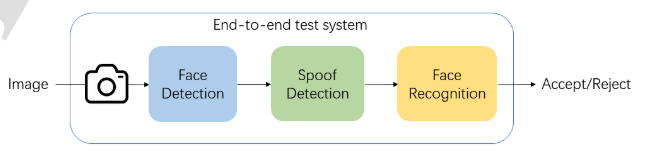
\includegraphics[width=0.6\textwidth]{img/report/Adversarial_attack_model}
	\caption{ساختار شبکه مورد استفاده برای یک سیستم تشخیص چهره\cite{Zhang2020}}
	\label{fig:Adverserial_Attack}
	\centering
\end{figure}

\newpage
برای مثال در مقاله (Zhang2020)
\cite{Zhang2020}
یک نوع از این حملات مورد بررسی قرار گرفتهٰاست. این حمله در بدترین سناریو یعنی زمانی که هکر از ساختار کلی شبکه با خبر است و هیچ دسترسی به سرور و محیط مدل و دادگان ندارد در نظر گرفته شده است.

در این روش هکر باید یک مدل مشابه با مدلی که قرار است به آن حمله صورت بگیرد درست کند و تصویر مد نظر را به مدل دهد خروجی آن را از مرحله تشخیص جعل بگیرد و با استفاده از روش های GAN جوری تصویر را تغییر دهد تا در مرحله بعد بتواند با تصویر مورد نظر سیستم را دور زده و دسترسی بگیرد. نکته حائز اهمیت در این سیستم‌ها این است یک فرآیند تبدیل داده از دیجیتال به آنالوگ و برعکس آن در فرآیند تصویر برداری از فرد و استفاده از تصویر گرفته شده در مدل است و این میتواند برای تولید داده توسط شبکه‌های GAN ایجاد مشکل کند زیرا باید بتواند بعد از تغییر از دیجیتال به آنالوگ و برعکس آن نیز ویژگی‌های مورد نیاز برای دور زدن سیستم را داشته باشد.

همانطور که در تصویر 
\ref{fig:Adverserial_Attack}
مشاهده می‌کنید شبکه از سه بخش تشخیص چهره، تشخیص جعل و شناسایی چهره تشکیل شده‌است. نکته حائز اهمیت این است که تصویر دستکاری شده باید از مرحله تشخیص چهره عبور کند، پس باید ساختار چهره در حین دستکاری حفظ شود. در تصویر
\ref{fig:Adverserial_Attack_schema}
مشاهده می‌کنید در این روش تصویر می‌بایست دوبار از فرياند تبدیل دیجیتال به آنالوک و برعکس عبور کند و می‌توان آن را نقص روش در نظر گرفت. با این‌ حال این روش می‌تواند موفقیت‌آمیز باشد و مدل کلی را دور بزند و به هکر اجازه ورود بدهد.

\begin{figure}[h]
	\centering
	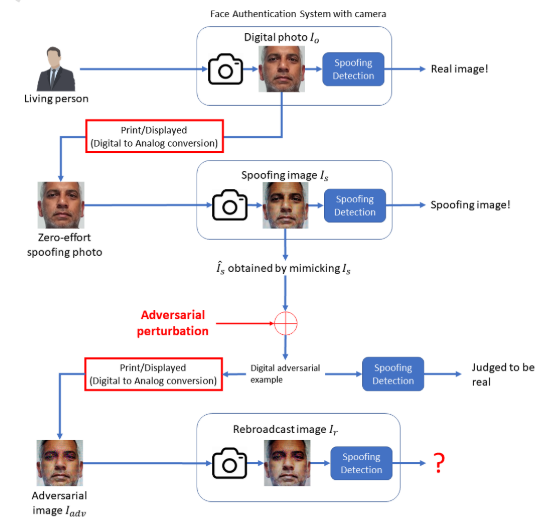
\includegraphics[width=0.6\textwidth]{img/report/Adversarial_attack_schema}
	\caption{ساختار حمله مورد استفاده برای یک سیستم تشخیص چهره\cite{Zhang2020}}
	\label{fig:Adverserial_Attack_schema}
	\centering
\end{figure}

\newpage
حملات درب پشتی را می‌توان در چند دسته قرار داد:
\cite{Guo2021}:
\begin{itemize}
	\item
	راه‌اندازی با استفاده از یک ورودی خاص (یک تصویر یا یک طرح خاص)
	\item
	نخریب فرآیند آموزش و دستکاری داده‌ها (مثلا در 
	\trans{MLaas}{Machine Learning as a Service}
	)
	\item
	انجام یک رفتار مخرب مانند: ناتوانی در دسته‌بندی تصویر ورودی یا کاهش دقت کلی مدل	
\end{itemize}

حملات درب پشتی میتوانند به صورت white-box یا black-box مبنی بر اینکه هکر درباره ساختار شبکه اطلاعات دارند و میتواند آن را تغییر دهد یا خیر. به طور مثال در مقاله (Guo2021)
\cite{Guo2021}
مدلی از حمله معرفی شده‌است که در آن فرض بر این است که هکر به تمامی فرآیند تسلط کامل دارد و با استفاده از یک تصویر و تغییر در ساختار دادگان تصاویر می‌تواند یک 
\trans{جعل هویت همگانی}{universal impersonate}
ایجاد کند و پس از آن به جای هر فردی احراز هویت شود.

این حمله نسبت به حملات مشابه قبلی از شدت بیشتری برخوردار است زیرا در حملات قبلی روی کاربر خاصی تمرکز می‌شد اما در این حمله تمرکز روی همه است و نکته دیگر درباره این حمله این است که این حمله بر روی شبکه سیامی تست شده است که ویژگی مهم این شبکه، مجموعه باز بودن فرآیند آموزش و آزمایش است. این شبکه یک ساختار دو قلو دارد و یک جفت تصویر را با هم مقایسه می‌کند برای ایجاد یک جعل هویت همگانی باید کاری کرد که شبکه در همه حالت درست کار کند مگر وقتی که تصویری را به عنوان ورودی بگیرد که هکر به آن داده است در این صورت باید همواره درست باشد و احراز هویت انجام شود.


برای این کار لازم است تا دادگان تصاویر تخریب شود و به ازای هر نمونه که چند تصویر وجود دارد با احتمال (نه خیلی کم که تصویر هکر شناخته نشود و نه زیاد که سیستم دچار اختلال شود.) تصاویر با تصویر هکر جایگزین شوند و برچسب ۱ مبنی بر مطابقت داشتن بگیرند. پس از آموزش شبکه با دادگان جدید هکر می‌تواند با ارسال تصویر خود به سیستم تشخیص چهره دسترسی لازم از سیستم را بگیرد. البته ممکن است نیاز باشد چندباری تلاش کند تا جواب صحیح بگیرد. (به دلیل کم بودن تعداد تصاویر هکر در مقایسه با تصاویر دادگان). برای توضیحات بیشتر مبنی بر نحوه ساخت دادگان و دادگان‌های استفاده شده و سایر موارد مقاله اصلی
\cite{Guo2021}
را مطالعه کنید. هدف از آوردن این مقاله در این بخش آشنایی بیشتر با انواع حملاتی بود که به سیستم‌های تشخیص چهره صورت میگیرد.

\section{جمع‌بندی}\label{sec:جمع‌بندی}
در بخش اول یادگیری با یک نمونه بررسی شد و شبکه سیامی که یکی از شبکه‌های پر کاربرد در تشخیص چهره است معرفی شد. در بخش دوم با یک مثال و بررسی‌های کلی در مورد یادگیری بدون نمونه سعی کردیم تا به طور کلی با این روش آشنا شویم. کاربرد روش بدون یادگیری بسیار گسترده‌است و از کاربرد‌های آن می‌توان به استفاده در تشخیص حرکت در ویدیو و جلوگیری از جعل هویت اشاره کرد. در بخش سوم کمی شبکه GAN را توضیح دادیم و چند مورد از حملات به سیستم‌های تشخیص چهره را توضیح دادیم. در ادامه و در فصل بعد کار‌های مرتبط انجام شده برای جلوگیری و تشخیص جعل تصویر چهره و حملات به این سیستم‌ها را بررسی می‌کنیم.
